\documentclass{beamer}

\mode<presentation> {
	
	% The Beamer class comes with a number of default slide themes
	% which change the colors and layouts of slides. Below this is a list
	% of all the themes, uncomment each in turn to see what they look like.
	
	%\usetheme{default}
	%\usetheme{AnnArbor}
	%\usetheme{Antibes}
	%\usetheme{Bergen}
	%\usetheme{Berkeley}
	%\usetheme{Berlin}
	%%%\usetheme{Boadilla}
	%\usetheme{CambridgeUS}
	%\usetheme{Copenhagen}
	%%%\usetheme{Darmstadt}
	%%%\usetheme{Dresden}
	\usetheme{Frankfurt}
	%\usetheme{Goettingen}
	%\usetheme{Hannover}
	%\usetheme{Ilmenau}
	%\usetheme{JuanLesPins}
	%\usetheme{Luebeck}
	%\usetheme{Madrid}
	%\usetheme{Malmoe}
	%%%\usetheme{Marburg}
	%%%\usetheme{Montpellier}
	%\usetheme{PaloAlto}
	%\usetheme{Pittsburgh}
	%\usetheme{Rochester}
	%\usetheme{Singapore}
	%\usetheme{Szeged}
	%\usetheme{Warsaw}
	
	% As well as themes, the Beamer class has a number of color themes
	% for any slide theme. Uncomment each of these in turn to see how it
	% changes the colors of your current slide theme.
	
	%\usecolortheme{albatross}
	%%%\usecolortheme{beaver}
	%\usecolortheme{beetle}
	%\usecolortheme{crane}
	%\usecolortheme{dolphin}
	%\usecolortheme{dove}
	%\usecolortheme{fly}
	%\usecolortheme{lily}
	%\usecolortheme{orchid}
	%\usecolortheme{rose}
	%\usecolortheme{seagull}
	%\usecolortheme{seahorse}
	%\usecolortheme{whale}
	%\usecolortheme{wolverine}
	
	%\setbeamertemplate{footline} % To remove the footer line in all slides uncomment this line
	\setbeamertemplate{footline}[page number] % To replace the footer line in all slides with a simple slide count uncomment this line
	
	\setbeamertemplate{navigation symbols}{} % To remove the navigation symbols from the bottom of all slides uncomment this line
}


\usepackage[utf8]{inputenc}
\usepackage[ukrainian]{babel}

\usepackage{amssymb}
\usepackage{physics}


\usepackage[active]{srcltx}
\usepackage[final]{pdfpages}

\usepackage{verbatim}

\usepackage{graphicx} % Allows including images
\usepackage{booktabs} % Allows the use of \toprule, \midrule and \bottomrule in tables

\numberwithin{equation}{section}

%------------------------------------------------

 \newcommand{\tabboxl}[2]{\parbox{#1}{\vspace{0.1cm} #2 \vspace{0.1cm} }}

\newcommand{\tabboxr}[2]{\parbox{#1}{\vspace{-0.3cm}
		\begin{flushright} #2 \end{flushright} \vspace{-0.3cm} }}

\newcommand{\tabboxc}[2]{\parbox{#1}{\vspace{-0.3cm}
		\begin{center} #2 \end{center} \vspace{-0.3cm} }}

\newcommand{\liml}{\lim\limits}
\newcommand{\suml}{\sum\limits}
\newcommand{\intl}{\int\limits}

\newcommand{\inttwopi}{\intl_{0}^{2\pi}}

\newcommand{\boundprob}{(\ref{laplace-eq}) -- (\ref{neumann-condition})}

\newtheorem{thm}{\protect\thmname}
\renewcommand{\thmname}{Теорема}

%----------------------------------------------------------------------------------------
%	TITLE PAGE
%----------------------------------------------------------------------------------------


\title[Short title]{Розробка алгоритмів захисту від атак на глибокі нейронні мережі} % The short title appears at the bottom of every slide, the full title is only on the title page

\author{Бугрій Богдан} % Your name
\institute[UCLA] % Your institution as it will appear on the bottom of every slide, may be shorthand to save space
{
	Львівський національний університет імені Івана Франка \\
	Факультет прикладної математики та інформатики 
}
\date{\today} % Date, can be changed to a custom date

\begin{document}
	%------------------------------------------------
	
	\begin{frame}
		\titlepage
	\end{frame}
	
	%------------------------------------------------
	
	\begin{frame}
		\frametitle{Зміст}
		\tableofcontents
	\end{frame}

	%------------------------------------------------
	\section{Опис проблеми}
	%------------------------------------------------
	
	\subsection{Постановка задачі}

	\begin{frame}
		\frametitle{Проблема}
		Нехай $M$ -- система машинного навчання, $x\in \mathbb{R}^n$ -- вхідний зразок, $y_{true}\in \mathbb{R}^C$ - правильне передбачення для зразка $x$, тобто 
		\begin{equation}
			M(x) = y_{true}
		\end{equation} 
		Можна створити зразок $x^{adv}=x+\tau$, де $\tau\in \mathbb{R}^n$, такий, що 
		\begin{equation}
			M(x^{adv})\neq y_{true}
		\end{equation}
	\end{frame}

	\begin{frame}
		\frametitle{Постановка задачі}
		Нехай $S^{adv}(M) \subset S$ -- множина ошукуючих зразків для моделі $M$. Необхідно знайти модель $M'$ таку, що
		\begin{equation}
			S^{adv}(M') = \emptyset.
		\end{equation}
		%Мається на увазі, що для моделі $M'$ неможливо створити ошукуючі зразки, тобто вона є невразливою до атак. 
		%Такий ``ідеальний'' випадок є практично неможливим, тому ми будемо використовувати пом'якшене формулювання, а саме вимагатимемо, щоб для моделі-образа задовільнялася умова
		На практиці модель-образа повинна задовільняти умову
		\begin{equation}
			n(S^{adv}(M')) < n(S^{adv}(M))
		\end{equation}
		де $n(S)$ --кількість елементів в множині $S$.
		% Іншими словами, нашою метою є побудова моделі, більш стійкої до атак, ніж оригінал.
	\end{frame}


	%-------------------------------------------------
	\subsection{Типи захисту}
	\begin{frame}
		\frametitle{Типи захисту}
		\begin{block} {За типом атак} 
			\begin{itemize}
				\item Захист від ошукуючих атак.
				\item Захист від викрадення.
				\item Захист від отруєння.
			\end{itemize}
		\end{block}
		\vspace{.5cm}
		\begin{block} {За стратегією захисту}
			\begin{itemize}
				\item Модифікація архітектури моделі та процесу тренування.
				\item Генерація специфічного тренувального набору.
				\item Створення захисної оболонки.
			\end{itemize}
		\end{block}	
	\end{frame}
	\begin{comment}
	\begin{columns}
	\begin{column}{.40\textwidth}
	\begin{block} {За типом атак} 
	\begin{itemize}
	\item захист від ошукуючих атак.
	\item захист від викрадення.
	\item захист від отруєння.
	\end{itemize}
	\end{block}	
	\end{column}
	\begin{column}{.40\textwidth}
	\begin{block} {За стратегією захисту}
	\begin{itemize}
	\item Модифікація архітектури моделі та процесу тренування.
	\item Генерація специфічного тренувального набору.
	\item Створення захисної оболонки.
	\end{itemize}
	\vspace{.85cm}
	\end{block}	
	\end{column}
	\end{columns}
	\end{comment}
	
	%------------------------------------------------
	\section{Ошукуючі зразки}
	%------------------------------------------------
	\subsection{}
	\begin{frame}
		\frametitle{Природа ошукуючих зразків}
		\begin{figure}[h]
			\centering
			
\includegraphics[width=.8\textwidth]{../images/six.png}
			
			%\caption{Область $D$}
			%\label{fig:double-connected-region}
		\end{figure}
	\vspace{1cm}
		\begin{center}
			\LARGE
			$x+\tau=x^{adv}$
		\end{center}
	\end{frame}
	
	\subsection{}
	\begin{frame}
		\frametitle{Атаки}
		
	\end{frame}


	%------------------------------------------------
	\section{Стійкість}
	\subsection{}
	\begin{frame}
		\frametitle{}
		\begin{columns}
			\begin{column}{.50\textwidth}
				Ідея, на якій базується визначення стійкості:
				 \begin{equation}
					\forall \tau \in B_{p}(L): \hat{y}_{k}(x+\tau)>\max _{i: i \neq k} \hat{y}_{i}(x+\tau)
				\end{equation}
				де $k:=M(x)$, $\hat{y}$ -- вектор ймовірностей.
				\vspace{0.2cm}
				
				Метрика для визначення стійкості:
				\begin{equation}
					\label{robustness-metric}
					r_p(M, X_{test}) := \frac{\sum\limits^{n_{test}}_{i = 1}\|x_i-x^{adv}_i\|_{p}}{n_{test}}
				\end{equation}
				де $n_{test}$ = $n(X_{test})$
				
			\end{column}
			
			\begin{column}{.50\textwidth}
				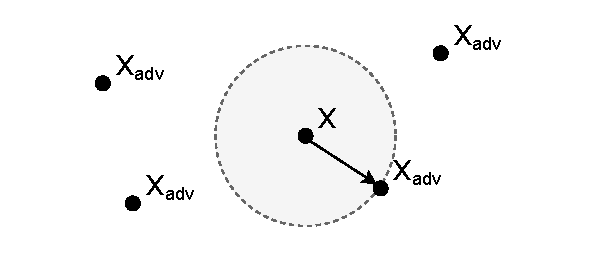
\includegraphics[width=0.45\paperwidth]{../images/2Dball.pdf}
			\end{column}
		\end{columns}
		
	\end{frame}
	\begin{comment}
	\begin{figure}[h]
	\centering
	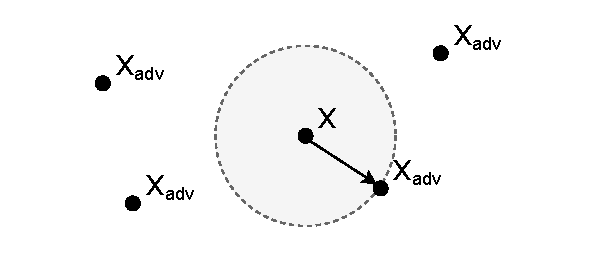
\includegraphics[width=1\textwidth]{../images/2Dball.pdf}
	
	%\caption{Область $D$}
	%\label{fig:double-connected-region}
	\end{figure}
	\end{comment}
	%------------------------------------------------
	
	
	%------------------------------------------------
	\section{Захисна дистиляція}
	\subsection{}
	\begin{frame}
		\frametitle{Ідея методу}
	
		\begin{figure}[h]
			\centering
			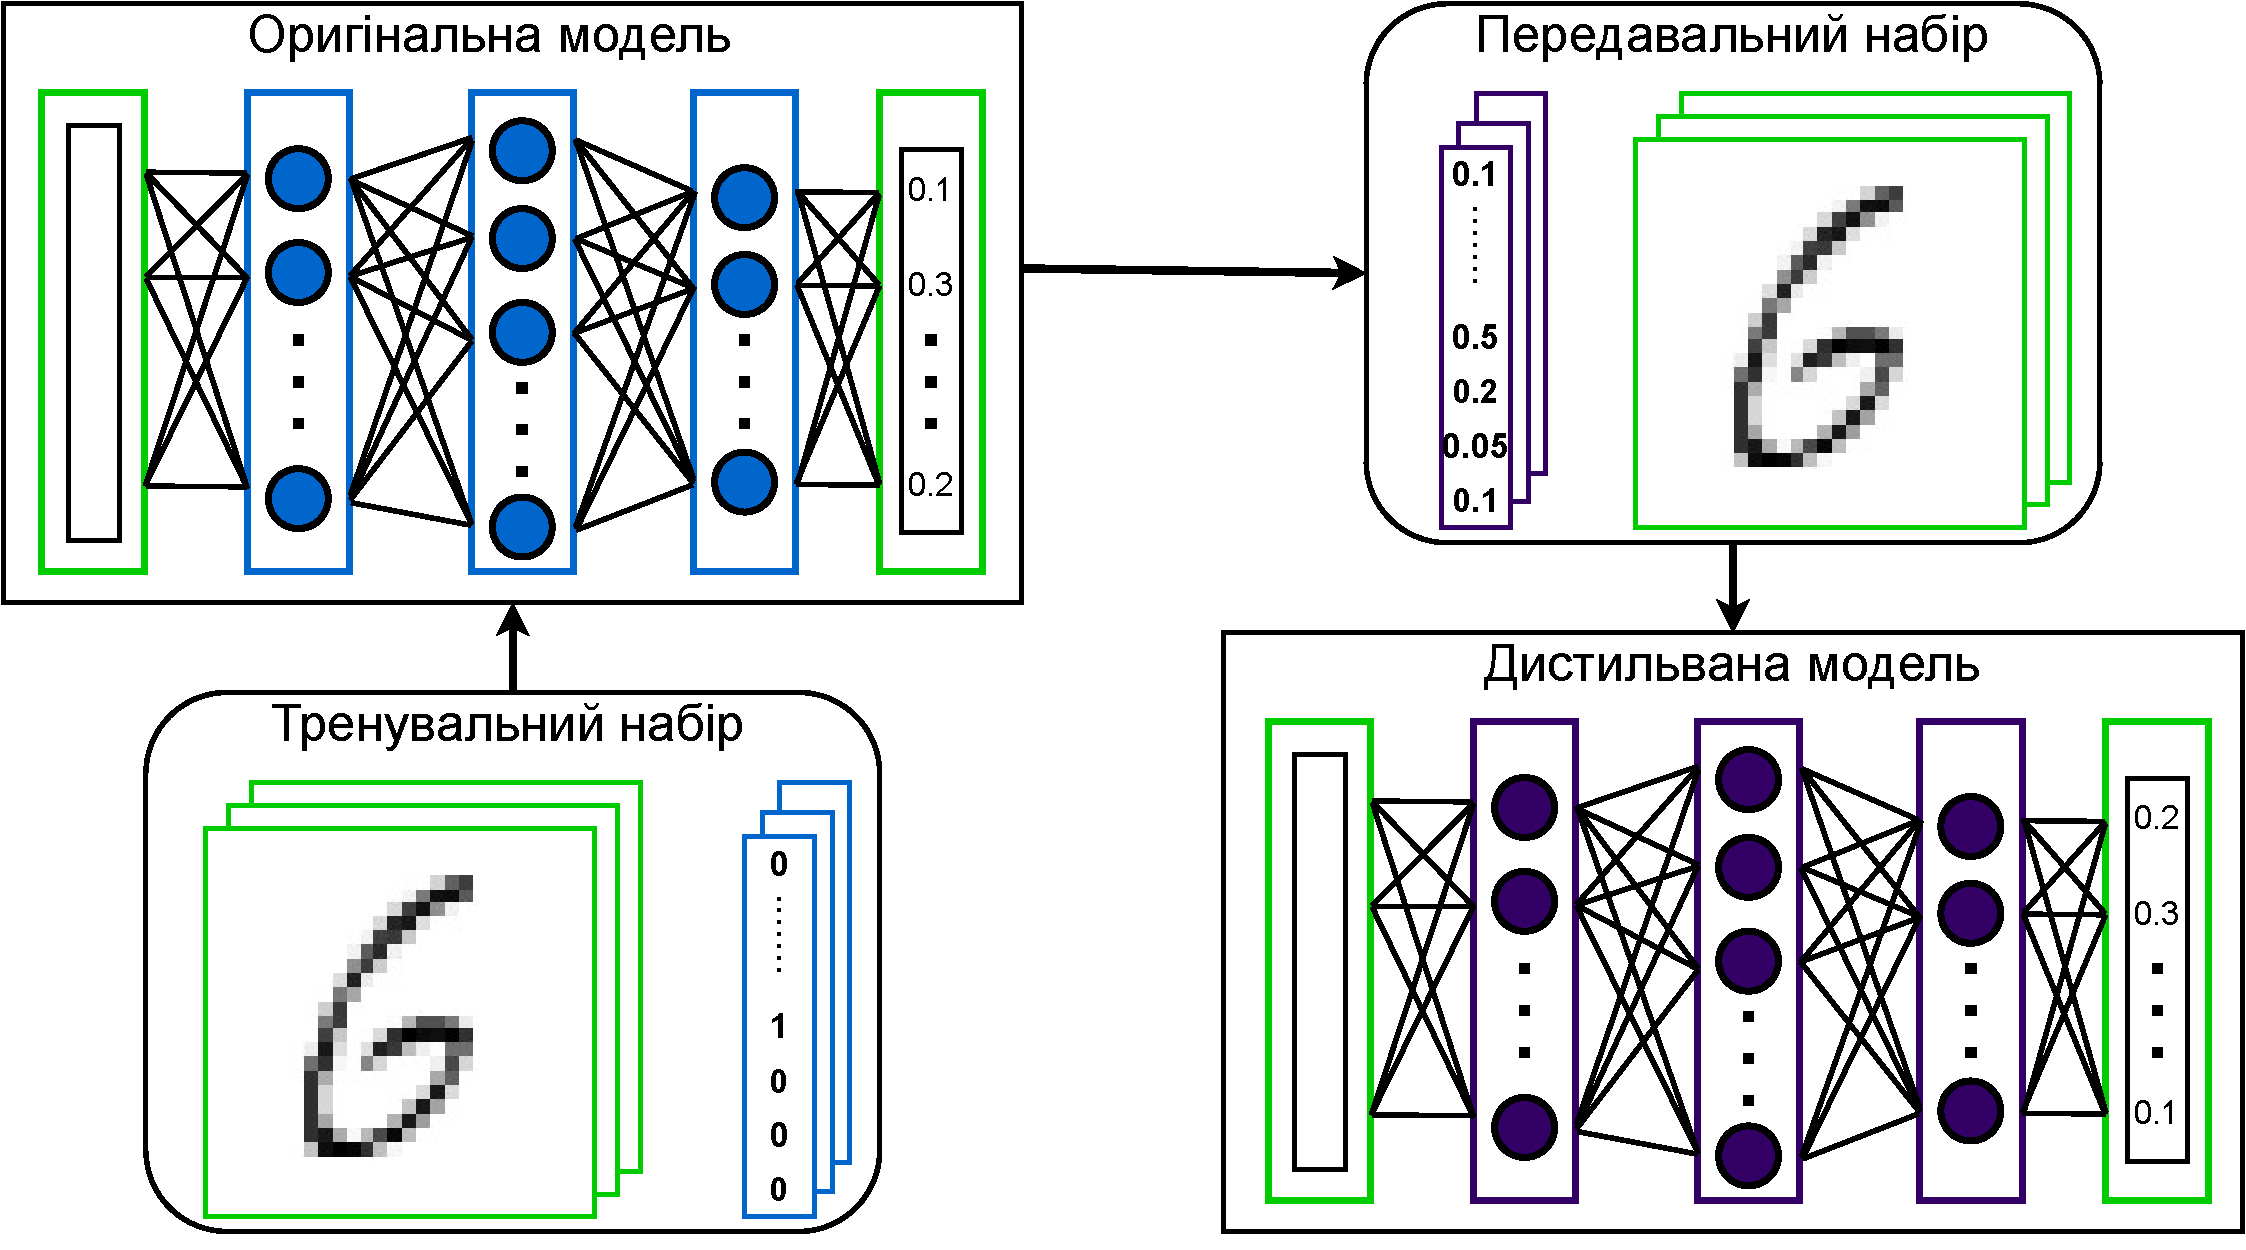
\includegraphics[width=1\textwidth]{../images/diagrams-Distillation.pdf}
			
			%\caption{Область $D$}
			%\label{fig:double-connected-region}
		\end{figure}
	\end{frame}

	\subsection{}
	\begin{frame}
		\frametitle{Основні параметри}
		
		Формула Softmax
		
		\begin{figure}[h]
			\centering
			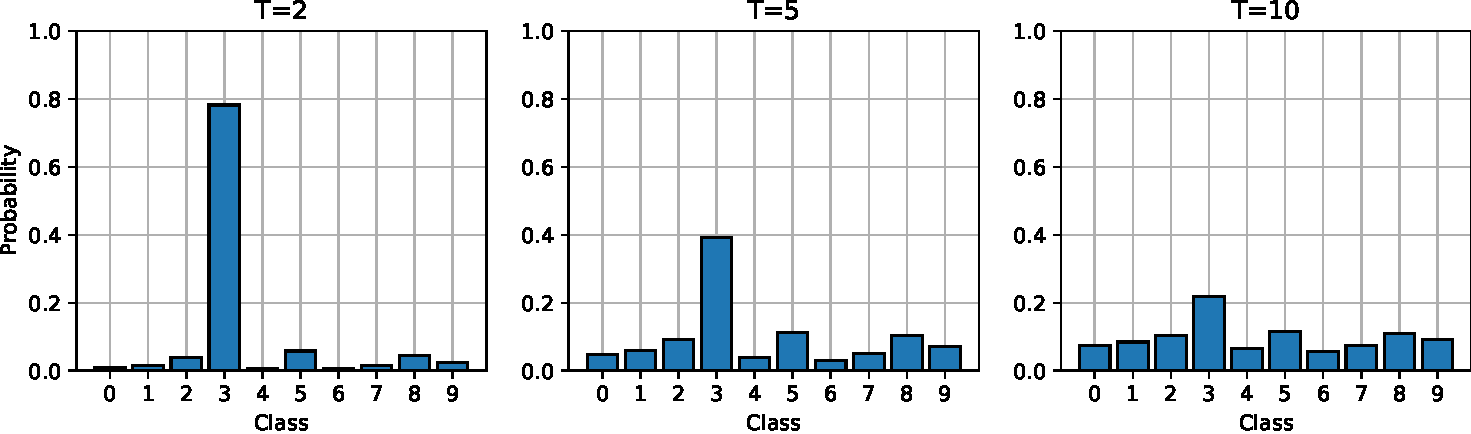
\includegraphics[width=0.6\textwidth]{../images/TvsP.pdf}
			
			%\caption{Область $D$}
			%\label{fig:double-connected-region}
		\end{figure}
	\end{frame}
	\subsection{}
	
	\begin{frame}
		\frametitle{Переваги та недоліки}
		
	\end{frame}
	%------------------------------------------------
	
	
	%------------------------------------------------
	\section{Захист PixelDP}
	\subsection{}
	\begin{frame}
		\frametitle{Ідея методу}
		
		\begin{figure}[h]
			\centering
			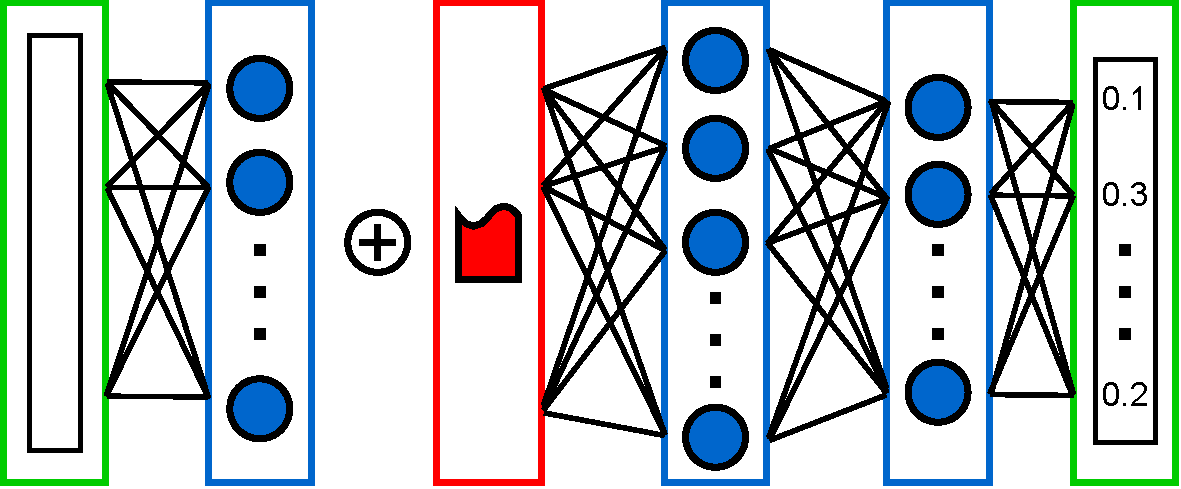
\includegraphics[width=0.6\textwidth]{../images/diagrams-PixelDP-small.pdf}
			
			%\caption{Область $D$}
			%\label{fig:double-connected-region}
		\end{figure}
	\end{frame}

	\subsection{}
	\begin{frame}
		\frametitle{Вимоги до архітектури}
		
	\end{frame}

	\subsection{}
	\begin{frame}
		\frametitle{Переваги та недоліки}
		
	\end{frame}

	
	%------------------------------------------------
	
	
	%------------------------------------------------
	\section{Експерименти}
	\begin{frame}
		\frametitle{Вплив параметрів на стійкість моделі}
		
		\begin{figure}[h]
			\centering
			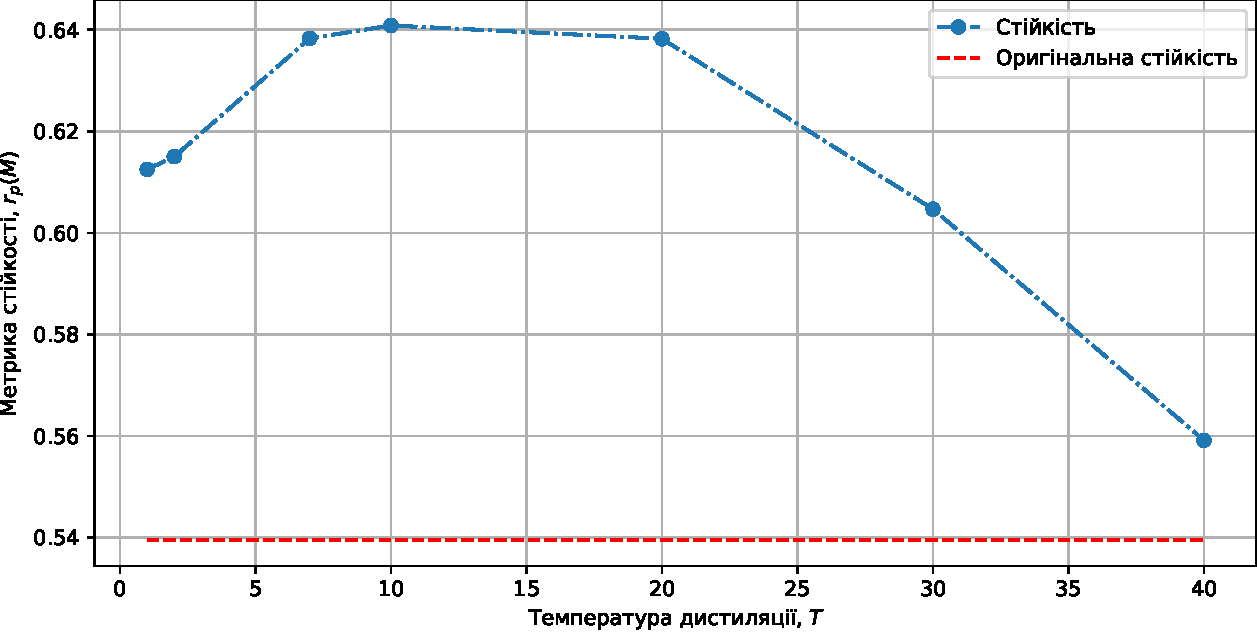
\includegraphics[width=0.6\textwidth]{../images/robustness.pdf}
			
			%\caption{Область $D$}
			%\label{fig:double-connected-region}
		\end{figure}
	
		Ключові зауваження і спостереження
	\end{frame}

	\begin{frame}
		\frametitle{Аналіз точності передбачень}
		\begin{center}
			\begin{tabular}{|c|c|c|c|c|}
				\hline
				\tabboxc{2.3cm}{$T$}
				& \tabboxc{2.3cm}{Точність на $X_{train}$}
				& \tabboxc{2.3cm}{Точність на $X_{test}$}
				& \tabboxc{2.3cm}{$r_p(M)$}
				& \tabboxc{2.3cm}{Приріст стійкості}
				\\ \hline
				
				2
				& 92\%
				& 92\%
				& 0.615
				& 14\%
				\\ \hline
				
				7
				& 90\%
				& 89\%
				& 0.638
				& 18.3\%
				\\ \hline
				
				10
				& 88\%
				& 87\%
				& 0.641
				& 18.8\%
				\\ \hline
				
				20
				& 78\%
				& 77\%
				& 0.639
				& 18.5\%
				\\ \hline
			\end{tabular}
		\end{center}
		Ключові зауваження і спостереження
	\end{frame}

	\begin{frame}

		\begin{figure}[h]
			\centering
			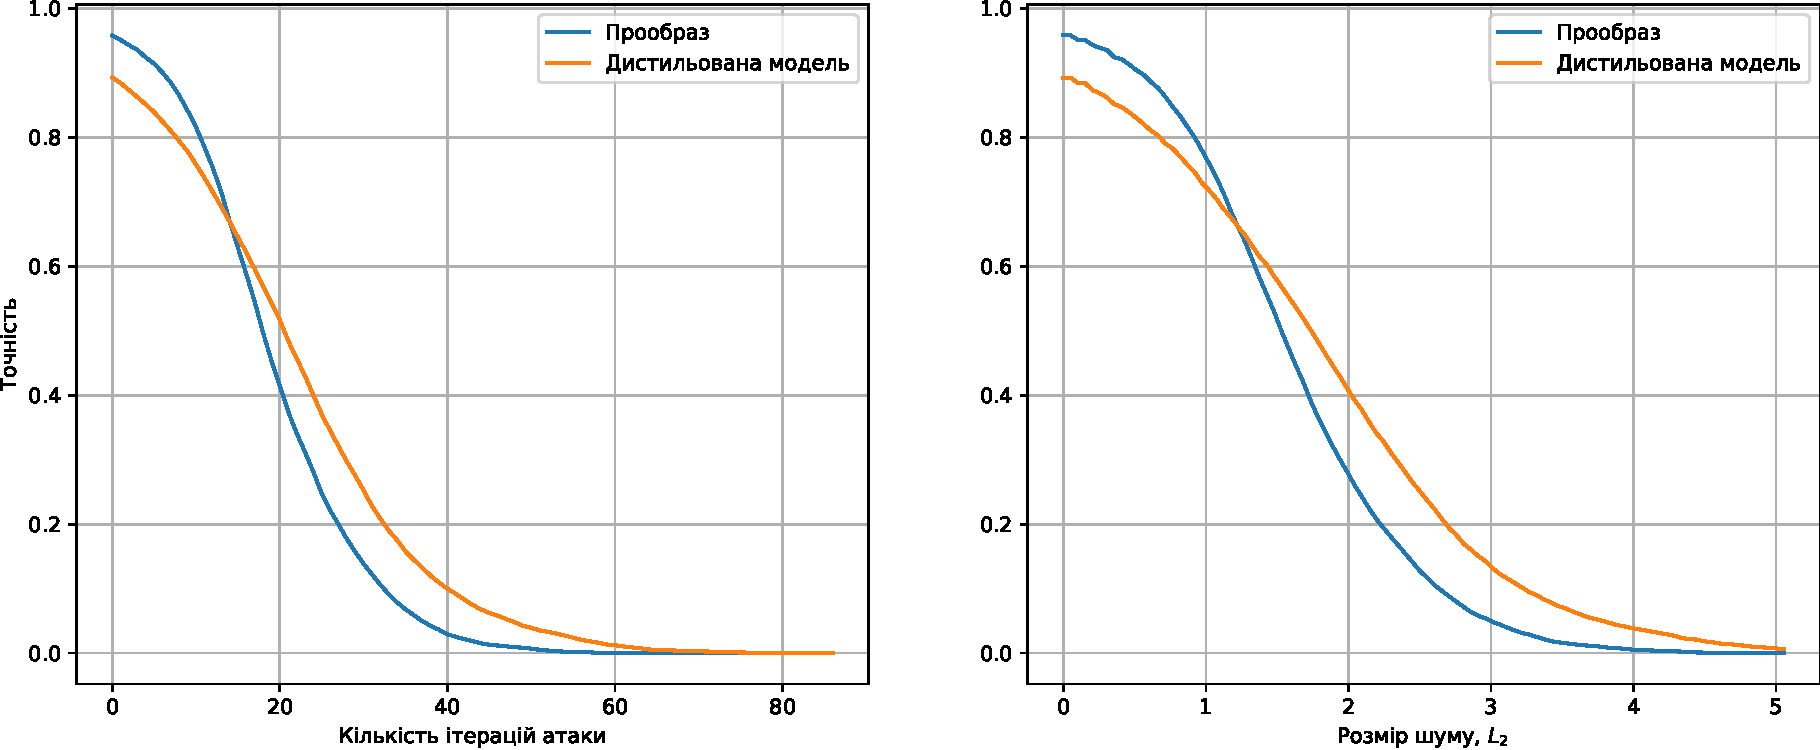
\includegraphics[width=0.6\textwidth]{../images/distAllT7.pdf}
			
			%\caption{Область $D$}
			%\label{fig:double-connected-region}
		\end{figure}
	
	    Ключові зауваження і спостереження
	\end{frame}

	
	%------------------------------------------------
	
	
	%------------------------------------------------
	\section{Висновки}
	%------------------------------------------------
	\begin{frame}
		\frametitle{Висновки}
		
		Наш вклад в роботу.
	\end{frame}
	
	
	
		
	\begin{frame}
		\frametitle{Текст}
		Текст
		\begin{figure}[h]
			\centering
			
\includegraphics[width=0.6\textwidth]{../images/empty.pdf}
			
			\caption{Область $D$}
			\label{fig:double-connected-region}
		\end{figure}
	\end{frame}
	
	\begin{frame}
		\frametitle{}
		\small
		%\textbf{\textit{Постановка задачі.}}
		Знайти функцію $u \in C^{2}(D)\bigcap  C^{1}(\overline{D})$ що задовольняє рівняння (\ref{laplace-eq}) та граничні умови (\ref{dirichlet-condition}), (\ref{neumann-condition})
	
		\begin{block}{}
			
			\begin{enumerate}
				\item
				Рівняння Лапласа: 
				\begin{equation}
					\label{laplace-eq}
					\Delta{u} = 0 \quad \text{в} \quad D
				\end{equation}
				
				\item
				Граничні умови:
				\begin{equation}
					\label{dirichlet-condition}
					u = f_1 \quad \text{на} \quad \Gamma_1,
				\end{equation}
				\vspace{-0.2cm}
				\begin{equation}
					\label{neumann-condition}
					\pdv{u}{\nu} = f_2 \quad \text{на} \quad \Gamma_2,		
				\end{equation}
		
			\end{enumerate}
		\end{block}
		де $\nu = \nu(x)$ - одиничний вектор зовнішньої нормалі, (\ref{dirichlet-condition}) називатимемо умовою Діріхле, а (\ref{neumann-condition}) -- умовою Неймана.

		
	\end{frame}
	\begin{comment}
		Розглядаємо мішану задачу Діріхле-Неймана для рівняння Лапласа.
	\end{comment}

	%------------------------------------------------

	\subsection{Єдиність розв'язку}
	\begin{frame}
		\frametitle{Єдиність розв'язку}
		
		\begin{block}{Теорема}
			Нехай $\Gamma_{1}, \Gamma_{2}$ -- гладкі границі, що належать класу $C^1$, обмежують двозв'язну область $D$. Тоді задача \boundprob \space має на $D$ не більше одного розв'язку.
		\end{block}
		
		\begin{block}{Доведення}
			\begin{enumerate}
				\item $\exists u_1, u_2 \in C^{2}(\overline{D}): u_1 \neq u_2 $
				\item $u^* = u_1 - u_2$
				\item Застосувати першу формулу Гріна
				\item Підставити граничні умови
			\end{enumerate}
			
		\end{block}

	\end{frame}
	\begin{comment}
	Від супротивного. Припустимо, що $\exists u_1, u_2 \in C^{2}(\overline{D}): u_1 \neq u_2 $ -- два різні розв'язки задачі \boundprob. Запишемо цю задачу для функції $u^* = u_1 - u_2$
	та застосуємо для її розв'язку першу формулу Гріна. Підставивши в отриманий вираз граничні умови та опираючись на неперервність функції $u^*$ в $\overline{D}$, легко бачити, що $u^*\equiv0 \Rightarrow u_1\equiv u_2$. Отримано суперечність
	\end{comment}

	%------------------------------------------------
	\section{Зведення до системи iнтегральних рiвнянь} 	
	%------------------------------------------------

	\subsection{Пов'язані поняття. Теорія потенціалів}
	\begin{frame}
		\frametitle{Пов'язані поняття. Теорія потенціалів}
		\begin{block}{Потенціал простого шару}
			$$
			u(x)=\intl_{\partial D} \varphi(y) \Phi(x, y) d s(y), \quad x \in \partial D
			$$
		\end{block}
		\vspace{0.8cm}
		\begin{block}{Похідна від потенціалу простого шару}
			$$
			\frac{\partial u_{\pm}}{\partial \nu}(x) =
			\intl_{\partial D} \varphi(y) \frac{\partial \Phi(x, y)}{\partial \nu(x)} d s(y) \mp \frac{1}{2} \varphi(x),
			\quad x \in \partial D
			$$
		\end{block}
	\end{frame}

	%------------------------------------------------

	\subsection{Загальний вигляд розв'язку}
	\begin{frame}
		\frametitle{Загальний вигляд розв'язку}
		
		\begin{block}{Передумови}
			\begin{itemize}
				\item Потенціал простого шару є гармонічною функцією
				\item Задача \boundprob зводиться до системи ІР
			\end{itemize}
		\end{block}
		\vspace{0.8cm}
		\begin{block}{Вигляд розв'язку}
			$$
			u(x) 
			= \intl_{\Gamma_1} \varphi_1(y) \Phi(x, y) d s(y)
			+ \intl_{\Gamma_2} \varphi_2(y) \Phi(x, y) d s(y)
			, \quad x \in D
			$$
		\end{block}
	\end{frame}

	\begin{frame}
		\frametitle{Система ІР}
		
		\begin{block}{}
			$$
			\left\{
			\begin{array}{l}
				\displaystyle
				\intl_{\Gamma_{1}} \varphi_1(y) \Phi(x, y) d s(y)
				+ \intl_{\Gamma_{2}} \varphi_2(y) \Phi(x, y) d s(y)
				= f_{1}(x), \quad x \in \Gamma_{1} 
				\\ [0.5cm]
				\displaystyle
				\intl_{\Gamma_{1}} \varphi_1(y) \frac{\partial \Phi(x, y)}{\partial \nu(x)} d s(y) \space +
				\\
				\displaystyle
				\qquad\qquad + \space \frac{1}{2}\varphi_2(x)
				+ \intl_{\Gamma_{2}} \varphi_2(y) \frac{\partial \Phi(x, y)}{\partial \nu(x)} d s(y)
				= f_{2}(x), \quad x \in \Gamma_{2}
			\end{array}\right.
			$$
		\end{block}
	\end{frame}

	%------------------------------------------------
	\section{Параметризацiя та виділення особливостей} 
	%------------------------------------------------
	

	%------------------------------------------------
	\subsection{Параметризацiя} 
	%------------------------------------------------

	%------------------------------------------------	
	\begin{frame}
		\frametitle{Параметризацiя}
		Припустимо, що кривi $\Gamma_{1}$ та $\Gamma_{2}$ заданi в параметричному виглядi:
		\begin{equation}
			\Gamma_{i} := \{ x_{i}(t) = (x_{i1}(t), x_{i2}(t)), \; t \in [ 0, 2\pi ] \} , \quad i = 1, 2
		\end{equation}
		\indent де $x_{i} : \mathbb{R} \rightarrow \mathbb{R}^2$, $2\pi$ періодична $\forall{t} \; \abs{x'(t)} > 0$ 
		
		Подамо систему в параметричному вигляді
		\begin{small}
			\begin{equation}
				\label{IE-parametrized-system}
				\left\{
				\begin{array}{l}
					\displaystyle
					\inttwopi \psi_1(\tau) K_{11}(t, \tau) d \tau
					+ \inttwopi  \psi_2(\tau) K_{12}(t, \tau) d \tau
					= 2\pi g_{1}(t)
					\\ [0.3cm]
					\displaystyle
					 \pi \frac{\psi_2(t)}{\abs{x'_{2}(t))}}
					+ \inttwopi \psi_1(\tau) K_{21}(t, \tau) d \tau
					+ \inttwopi  \psi_2(\tau) K_{22}(t, \tau) d \tau
					= 2\pi g_{2}(t)
				\end{array}\right.
			\end{equation}
		
		де $\displaystyle \psi_{i}(t) = \varphi(x_{i}(t)) \abs{x'_{i}(t)}, \; g_{i} = f_{i}(x_{i}(t)), \;  i  = 1, 2; \; t \in [0, 2\pi]$ \\[0.3cm]
		
		\end{small}
	\end{frame}
	
	%------------------------------------------------
		

	
	%------------------------------------------------


	%------------------------------------------------
	\section{Чисельне розв'язування} 
	%------------------------------------------------

	\subsection{Метод колокації}
	\begin{frame}
		\frametitle{Метод колокації}
		
		\begin{block}{Розбиття та базисні функції}
			\begin{itemize}
			\item $x_{j}=a+j h, j=0, \ldots, n$, $h=(b-a) / n$
			\vspace{0.3cm}
			\item $X_{n}-$ простір функцій, неперервних на $[a, b]$
			\item $l_{j}(x)=\left\{
			\begin{array}{lc}
				\frac{x-x_{j-1}}{h}, \quad x \in\left[x_{j-1}, x_{j}\right], j \geq 1 \\
				\frac{x_{j+1}-x}{h}, \quad x \in\left[x_{j}, x_{j+1}\right], j \leq n-1 \\
				0, \qquad\quad \text { в інших випадках }
			\end{array}\right.$
		
			\end{itemize}
		\end{block}
		
		\begin{block}{Вигляд наближеного розв'язку}
		$$
		\tilde{\psi_k}(x)=\sum_{j=1}^{n} c^{(k)}_{j} l_{j}(x), \quad k = 1, 2
		$$
		\end{block}
		

	\end{frame}

	

	\begin{frame}
		\frametitle{Результуюча СЛАР}
		
		\begin{block}{}
			\Large
			$$
			Ac=g
			$$	
		\end{block}
		
		\begin{block}{}
		$$
		\begin{pmatrix}
			\begin{matrix}
				G^{(1)}_{11} & \dots  & G^{(1)}_{1n} \\
				\vdots 		 & \ddots & \\
				G^{(1)}_{n1} & 		  & G^{(1)}_{nn} \\
			\end{matrix} &
			\begin{matrix}
				G^{(2)}_{11} & \dots  & G^{(2)}_{1n} \\
				\vdots 		 & \ddots & \\
				G^{(2)}_{n1} & 		  & G^{(2)}_{nn} \\
			\end{matrix} \\[1cm]
			\begin{matrix}
				G^{(3)}_{11} & \dots  & G^{(3)}_{1n} \\
				\vdots 		 & \ddots & \\
				G^{(3)}_{n1} & 		  & G^{(3)}_{nn} \\
			\end{matrix} &
			\begin{matrix}
				G^{(4)}_{11} & \dots  & G^{(4)}_{1n} \\
				\vdots 		 & \ddots & \\
				G^{(4)}_{n1} & 		  & G^{(4)}_{nn} \\
			\end{matrix} \\
		\end{pmatrix}
		\begin{pmatrix}
			c^{(1)}_1\\
			\vdots\\
			c^{(1)}_n\\[0.5cm]
			c^{(2)}_1\\
			\vdots\\
			c^{(2)}_n\\
		\end{pmatrix}
		= 
		\begin{pmatrix}
			2\pi g_1(x_1)\\
			\vdots\\
			2\pi g_1(x_n)\\[0.5cm]
			2\pi g_2(x_1)\\
			\vdots\\
			2\pi g_2(x_n)\\
		\end{pmatrix}
		$$
		\end{block}
		
	\end{frame}
		
	%------------------------------------------------
	
	\subsection{Похибка}	
	\begin{frame}
		\frametitle{Похибка}
	
		\begin{block}{Проекційний оператор }
		$$
		\left(P_{n} \varphi\right)(x)= \sum_{j=0}^{n} \varphi\left(x_{i}\right) l_{j}(x) .
		$$
		\end{block}
		
		Для $P_{n} \varphi$ маємо такі оцінки 
		$$
		\begin{array}{l}
			\displaystyle
			\varphi \in C^{2}[a, b], \quad \quad \left\|P_{n} \varphi-\varphi\right\|_{\infty} \leq \frac{1}{8} h^{2}\left\|\varphi^{\prime \prime}\right\|_{\infty}  
			\\[0.3cm]
			
			\displaystyle
			\varphi \in C[a, b], \quad \quad \left\|P_{n} \varphi-\varphi\right\|_{\infty} \leq w(\varphi, h) \rightarrow 0
		\end{array}
		$$
		
	
	\begin{block}{Оцінка похибки}
		$$
		\left\|\varphi_{n}-\varphi\right\|_{\infty} \leq M \frac{1}{8} h^{2}\left\|\varphi^{\prime \prime}\right\|_{\infty}, \quad \text{для } 
		\varphi \in C^{2}[a, b]
		$$
	\end{block}	
			
		
		
	\end{frame}
	
	%------------------------------------------------

	\section{Чисельні експеременти} 

	\begin{frame}
		\frametitle{Приклад 1.}
				
					
		
		{\small{
		\begin{equation}
			\label{ex1}
			\begin{array}{l}
				\displaystyle
				\Gamma_{1}=\left\{x_{1}(t)=(0.9 \cos t, 0.9 \sin t), \quad t \in[0,2 
				\pi]\right\} \\
				
				\displaystyle
				\Gamma_{2}=\left\{x_{2}(t)=(2 \cos t, 2 \sin t), \quad  t \in[0,2 \pi]\right\} \\[0.1cm]

				\displaystyle
				f_{1}(x)=x  \text { на } \Gamma_{1} \quad \text {і} \quad
				f_{2}(x)=1  \text { на } \Gamma_{2}
			\end{array}
		\end{equation}
		}}
				
		\begin{figure}
			
\includegraphics[width=0.48\textwidth]{../images/empty.pdf}
			\caption{Граничні умови $\Gamma_1$, $\Gamma_2$ для \ref{ex1}}
		\end{figure}
		
	\end{frame}

	

	\begin{frame}
		\begin{columns}[c] 
			\column{.5\textwidth}
			\begin{figure}
				
\includegraphics[width=1\textwidth]{../images/empty.pdf}
				\caption{Точний розв'язок}	
			\end{figure}
						
			\column{.5\textwidth}
			\begin{figure}
				
\includegraphics[width=1\textwidth]{../images/empty.pdf}
				\caption{Наближений розв'язок}
			\end{figure}
						
		\end{columns}
		
	\end{frame}	
	

	%------------------------------------------------
	
\section*{Література}
\begin{frame}
	\thispagestyle{empty}
	\frametitle{Література}
	\begin{thebibliography}{99}
		

		\bibitem[1]{defencive-distillation}
		\textit{Nicolas Papernot, Patrick McDaniel, Xi Wu Somesh Jha,Ananthram Swami} /
		Distillation as a Defense to Adversarial Perturbations against Deep Neural Networks /
		arXiv preprint arXiv:1511.04508 (2016)
		
		\bibitem[2]{pixeldp}
		\textit{Mathias Lecuyer, Vaggelis Atlidakis, Roxana Geambasu, Daniel Hsu, Suman Jana} /
		Certified Robustness to Adversarial Examples with Differential Privacy/
		arXiv preprint arXiv:1802.03471 (2019)
		
		\bibitem[3]{analysis-of-robustness}
		\textit{Alhussein Fawzi, Omar Fawzi, Pascal Frossard} /
		Analysis of classifiers' robustness to adversarial perturbations /
		arXiv preprint arXiv:1502.02590 (2016)
		
		\bibitem[4]{my-work}
		\textit{Богдан Бугрій} /
		Атаки на глибокі нейронні мережі /
		Львів (2020)
		
		
	\end{thebibliography}
\end{frame}

\end{document} 